This exercise focuses on red eye removal from a picture (in this case, the picture on \autoref{fig:ex4-before}).
The specified sequence of steps is to start out by computing a score for each pixel that estimates the likelihood of that pixel belonging to a read eye (high score more likely).
The score is known as normalized cross-correlation and is expressed naturally as a stencil operation.
This score has already been computed in the exercise and the next step is therefore to sort these scores in ascending order (likelihood) effectively.
The final step is to reduce the redness of the highest scoring pixels and this can be performed using simple map operations.
As stencil and map operations have already been worked on in previous exercise, the focus of this exercise is to perform the sorting efficiently.
The result of the red eye removal can be seen in \autoref{fig:ex4-after}.
\begin{figure}[ht]
	\centering
	\begin{subfigure}{.5\textwidth}
		\centering
		\fbox{
			
\includegraphics[width=0.4\textwidth]{figs/exercises/ex4/red_eye_effect_5.jpg}
		}
		\caption{Before}
		\label{fig:ex4-before}
	\end{subfigure}%
	\begin{subfigure}{.5\textwidth}
		\centering
		\fbox{
			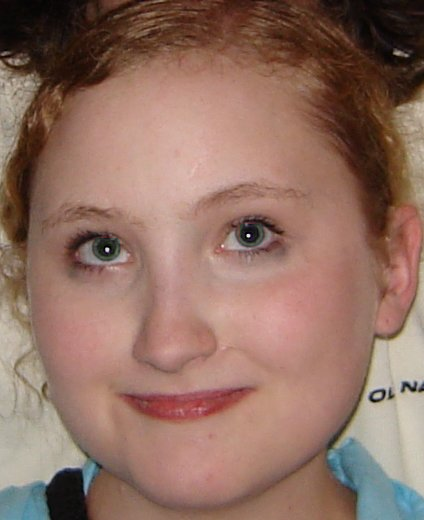
\includegraphics[width=0.4\textwidth]{figs/exercises/ex4/HW4_output.png}
		}
		\caption{After}
		\label{fig:ex4-after}
	\end{subfigure}
	\caption{Picture before and after red eye removal}
	\label{fig:ex4}
\end{figure}

The actual exercise is to implement a parallel radix sort as described in \autoref{sec:al_sort_radix}.
To compute the sort, a lot of work has to be done (the actual source code can be seen in \cite{exercises}.)
The following sequence of techniques are performed for every bit of the values to sort (32bit values in this exercise).
The steps are visualized in \autoref{fig:ex4-radix-sort}.
\begin{enumerate}
	\item[\textbf{Step 1}]
	An exclusive prefix sum scan is performed over a "vector" of predicates (ones or zeros).
	This is done for both the zeros and ones to sort.
	For the ones to sort, the predicate is true if the bit is one and false if it is zero, and the other way around (inverted) for the zeros to sort.
	It is used to determine the scattering offset address.
	Because the number of elements to sort is larger than the maximum number of threads in a thread block, the kernel must be executed using multiple thread blocks.
	As it is only possible to synchronize threads within a block, the resulting scan is actually a segmented scan, which is not the desired operation in this context.
	\item[\textbf{Step 2}]
	Because of the segmented scan operation, it is necessary to store the highest scattering offset address, and use this later to convert the segmented scan to a regular scan. 
	\item[\textbf{Step 3}]
	An exclusive prefix sum scan is performed on the elements stored from \textbf{Step1} to generate the offset value which should be added to the elements of the segmented scan.
	\item[\textbf{Step 4}]
	A histogram of the number of ones and zeros are generated.
	\item[\textbf{Step 5}]
	An exclusive prefix sum scan is performed over the histogram.
	This is to generate the scattering offset to where the zeros and ones should start in the resulting vector.
	\item[\textbf{Step 6}]
	In the last step, the results of the precious steps are used to generate the resulting vector of sorted ones and zeros.
	The result from \textbf{Step 4} determines the start offset for zeros (0) and ones (7).	
	The value on index "blockId" from the result in \textbf{Step 2} is added to all elements in each block of the segmented scan from \textbf{Step 0}.
	When this is performed for both zeros and ones, the resulting vector contains the sorted zeros and ones.
\end{enumerate}
\begin{figure}[ht]
	\centering
	\fbox{
		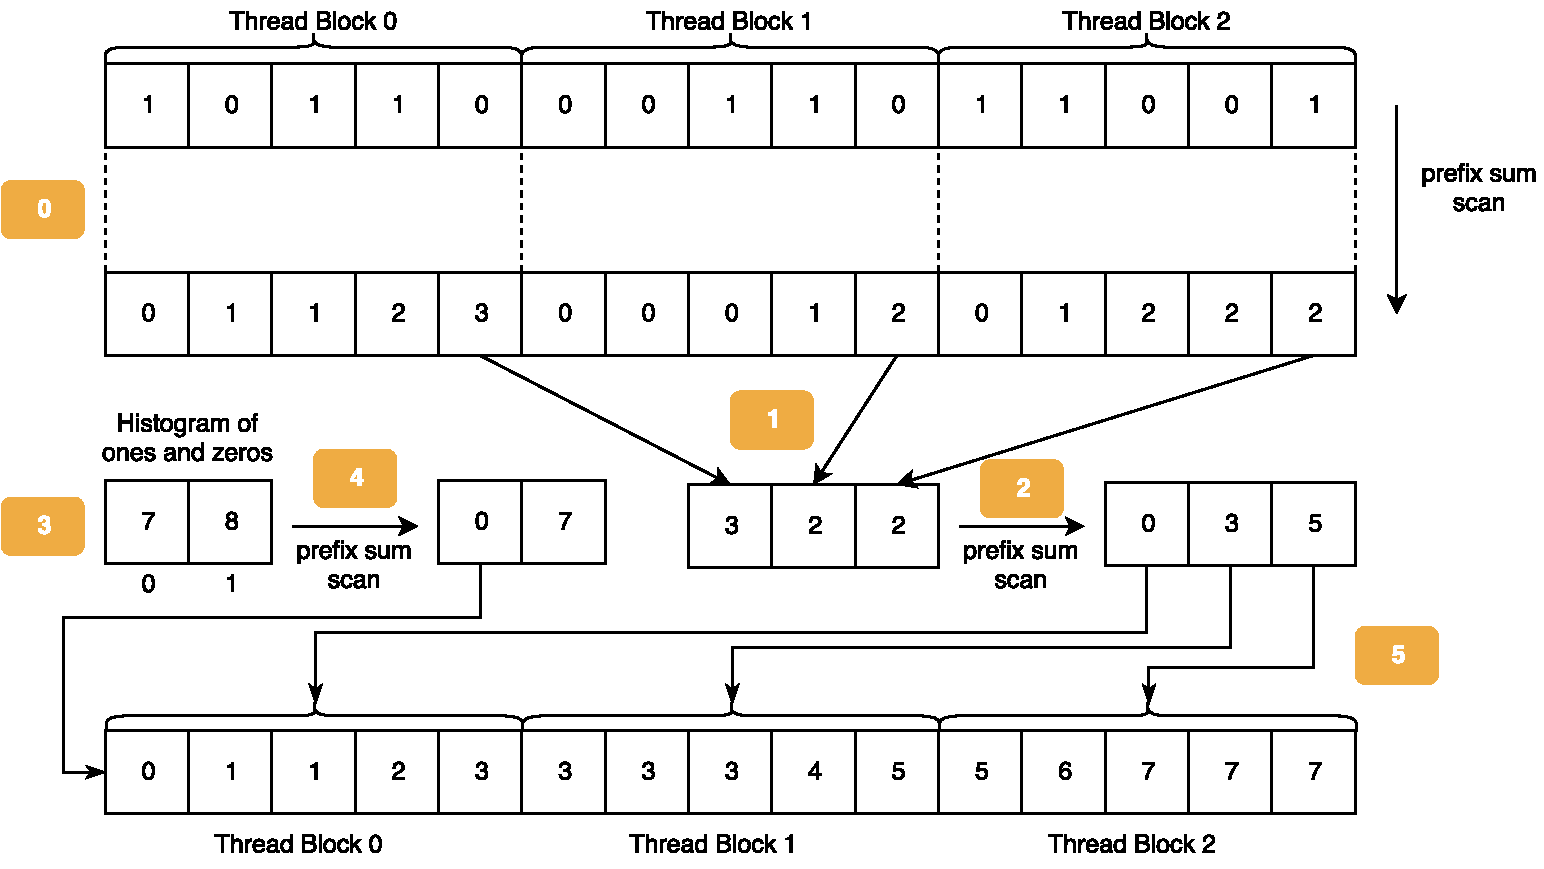
\includegraphics[width=1.0\textwidth]{figs/programming-model/ex4-radix-sort.pdf}
	}
	\caption{Exercise 4 radix sort implementation}
	\label{fig:ex4-radix-sort}
\end{figure}
%For every bit, starting a LSB, a histogram of the number of occurrences of each digit (0 or 1)
%Exclusive prefix sum scan of histogram
%predicate kernel (return vector with 1 for all ones and a vector with 1 for all zeros)
%Exclusive prefix sum scan of predicates, exclusive prefix sum scan of incr values and add kernel at the end
%move kernel, move to position if predicate is one
%swap input and output (out of order sort)